% Options here are passed to the article class.
% Most common options: 10pt, 11pt, 12pt
\documentclass[10pt]{datasheet}

% Input encoding and typographical rules for English language
\usepackage[utf8]{inputenc}
\usepackage[english]{babel}
\usepackage[english]{isodate}

% tikz is used to draw images in this example, but you can
% also use \includegraphics{}.
\usepackage{graphicx}

% These define global texts that are used in headers and titles.
\title{LC02: Hopperspeed Hex to Binary}
\author{Andrews54757}
\tags{logic-and-computation, converter}
\date{December 2022}
\revision{Revision 1}
\begin{document}
\maketitle

\section{Features}

\begin{itemize}
\item{Hopperspeed throughput}
\item{Stateless, uses quasi-based logic}
\item{14gt Latency}
\end{itemize}

\section{Applications}

\begin{itemize}
\item{Converting hex coded signals to binary}
\end{itemize}

\section{General Description}
The LC02 Hopperspeed Hex to Binary takes a hex coded signal and outputs a binary coded signal. It is hopperspeed, meaning it can be used to convert a hex coded signal to a binary coded signal every 8 game ticks.
\vfill\break

\begin{figure}[h]
    \centering
    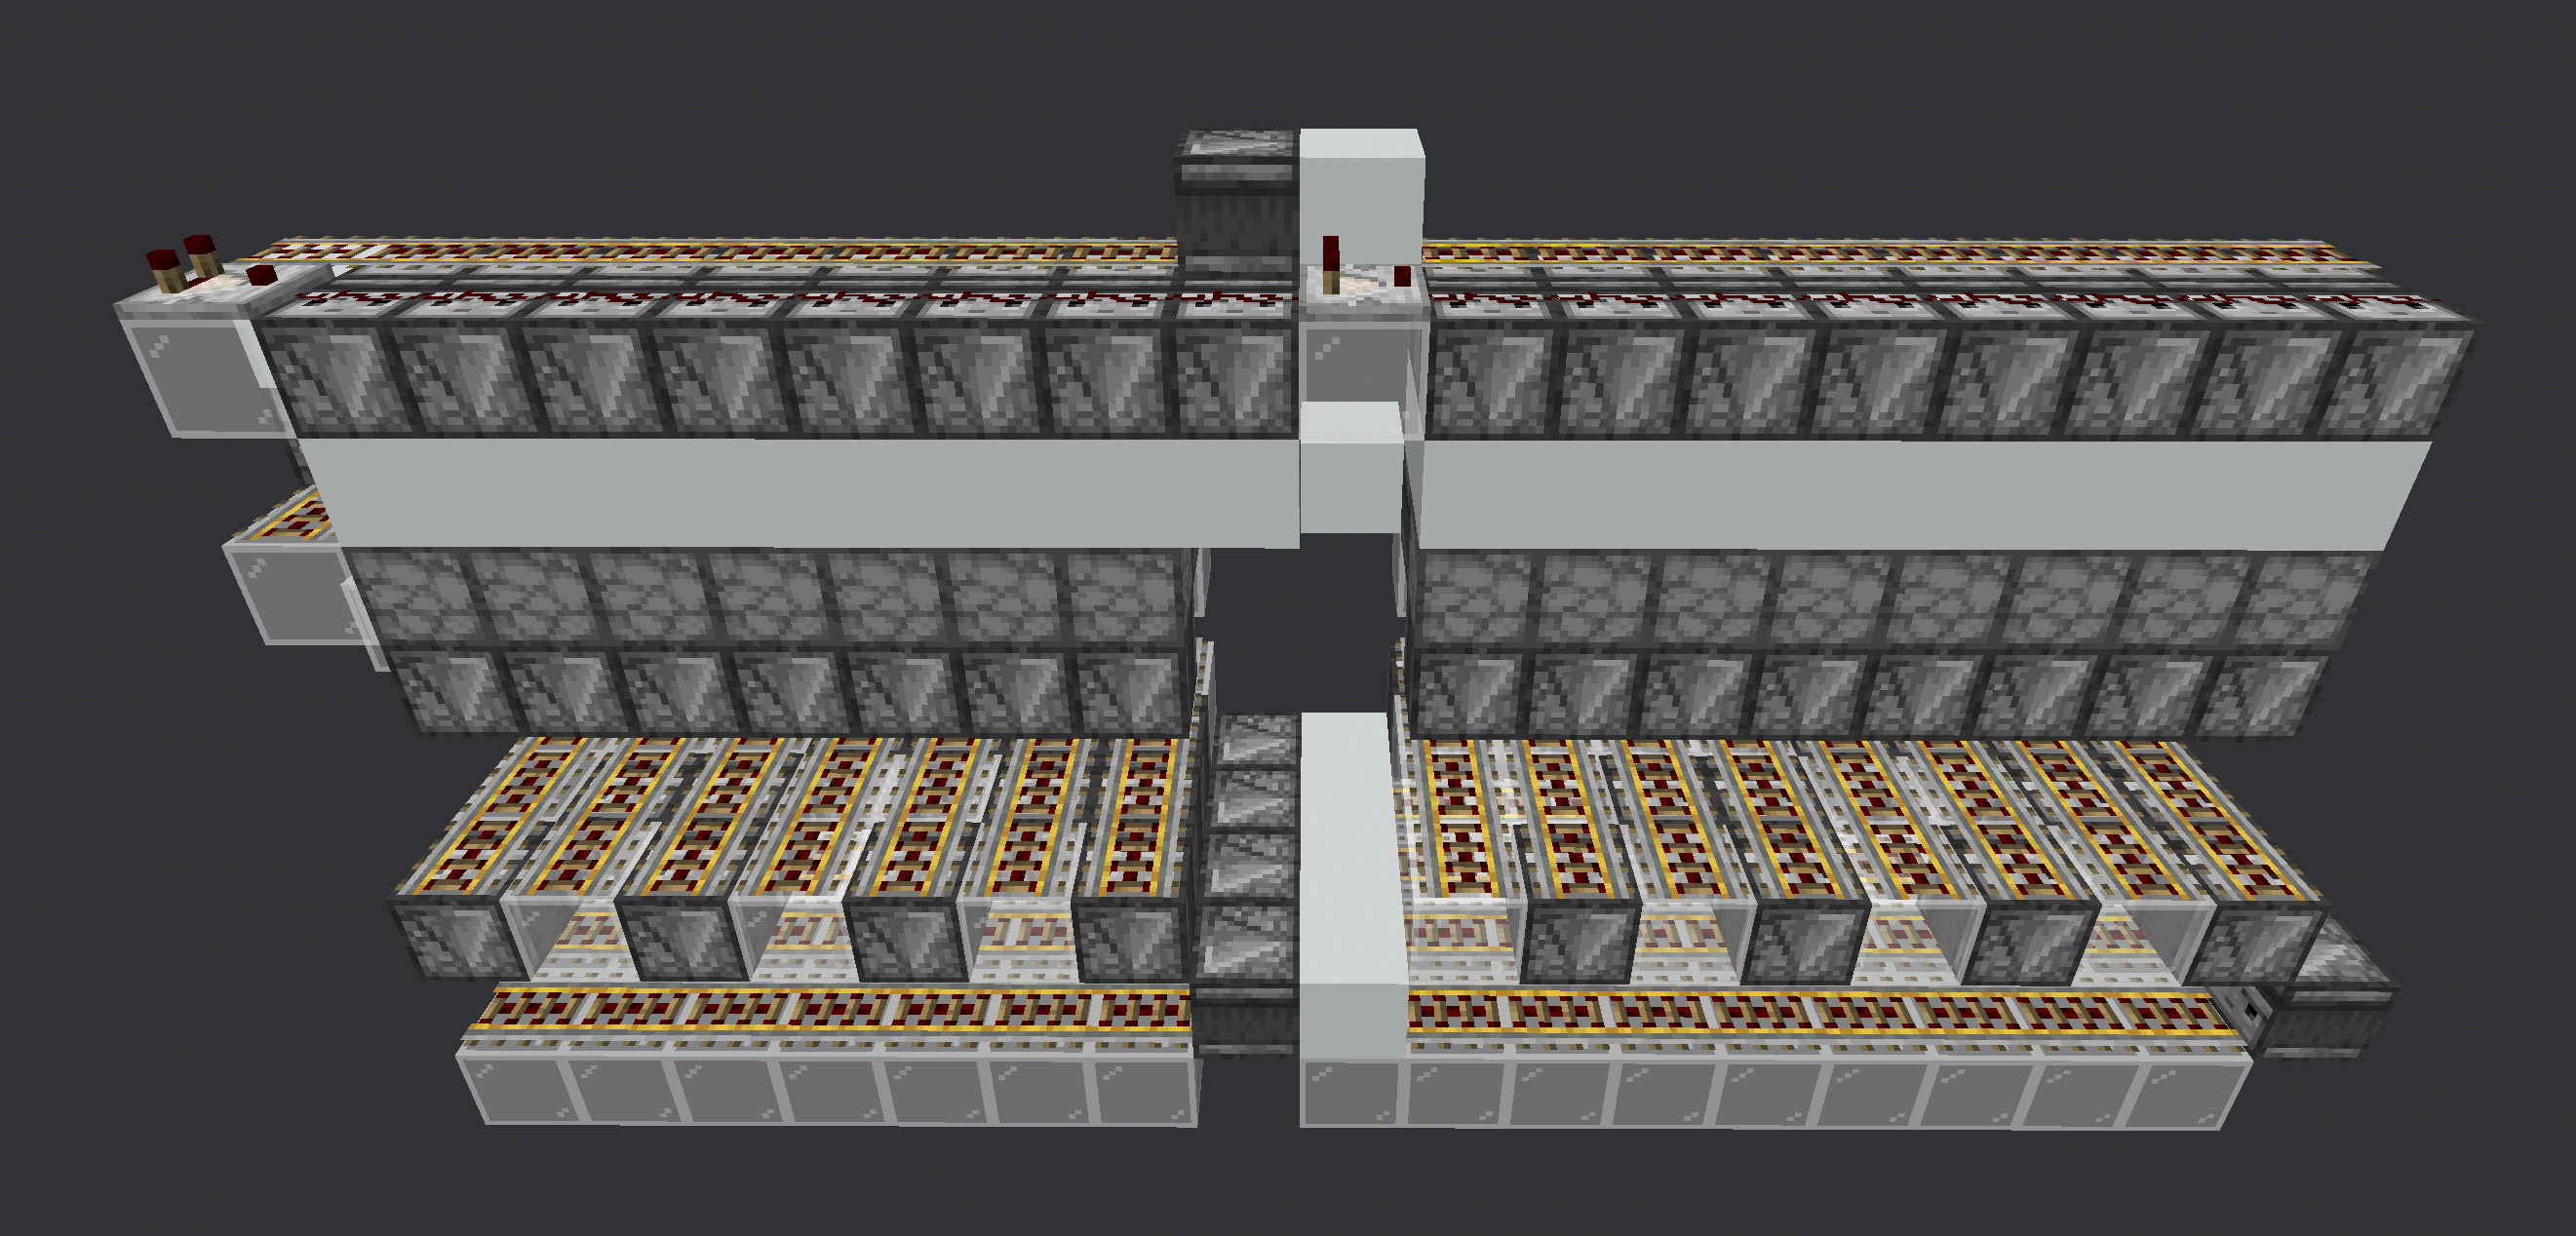
\includegraphics[width=0.48\textwidth]{hextobin.png}
    \caption{\centering Hopperspeed Hex to Binary}
\end{figure}

% For wide tables, a single column layout is better. It can be switched
% page-by-page.
\onecolumn

\section{Device Specifications}

\begin{table}[h]
    \caption{Inputs}
    \begin{tabularx}{\textwidth}{l | c | X}
        \thickhline
        \textbf{Name} & \textbf{Range} & \textbf{Description} \\
        \hline
        Signal input & 1-15 & Pulsed analog signal. \\
        \thickhline
\end{tabularx}
\end{table}

\begin{table}[h]
    \caption{Outputs}
    \begin{tabularx}{\textwidth}{l | c | X}
        \thickhline
        \textbf{Name} & \textbf{Range} & \textbf{Description} \\
        \hline
        Output bit0 & Pulse & First bit of converted signal \\
        Output bit1 & Pulse & Second bit of converted signal \\
        Output bit2 & Pulse & Third bit of converted signal \\
        Output bit3 & Pulse & Fourth bit of converted signal \\
        \thickhline
\end{tabularx}
\end{table}

\begin{table}[h]
    \caption{Device Specifications}
    \begin{tabularx}{\textwidth}{l | c c c | c | X}
        \thickhline
        \textbf{Parameter} & \textbf{Min.} & \textbf{Typ.} & \textbf{Max.} &
        \textbf{Unit} & \textbf{Conditions} \\
        \hline
        Throughput  & 8 & - & - & gt & Normal Usage \\
        \hline
        Latency    & 14 & - & - & gt & From input to output \\
        \hline
        MC Version & 1.13 & 1.17.1 & - & MCV & Latest version at time of writing: 1.19.3\\
        \hline
        Dimensions & & 19 x 9 x 4 & & Blocks & \\
        \thickhline
\end{tabularx}
\end{table}
\newpage
\section{Testing Data}
\begin{table}[h]
\caption{Executed Tests}
\begin{tabularx}{\textwidth}{l | X}
    \thickhline
    \textbf{Test} & \textbf{Result} \\
    \hline
    Conversion test & Device was able to convert signals successfully at 10gt throughput. \\
    \thickhline
\end{tabularx}
\end{table}

\section{Download Information}
\begin{table}[h]
    \caption{Download Information}
    \begin{tabularx}{\textwidth}{l | l | l | X}
        \thickhline
        \textbf{Identifier} & \textbf{MC} & \textbf{File} & \textbf{Description} \\
        \hline
        LC02 & 1.17.1 & \href{https://github.com/Soontech-Annals/Archive/blob/364bde8dbcbc2e5337489ff435bcda9b387017e2/Archive/logic-and-computation/LC02\%20Hopperspeed\%20Hex\%20to\%20Binary/LC02\_hopperspeed\_hex\_to\_bin.litematic?raw=1}{LC02\_hopperspeed\_hex\_to\_bin.litematic} & Schematic of device. \\
        \hline
        \thickhline
    \end{tabularx}
\end{table}

\end{document}

